%{{{ Formatierung

\documentclass[a4paper,10pt]{article}

\usepackage{physics_notetaking}

%%% dark red
%\definecolor{bg}{RGB}{60,47,47}
%\definecolor{fg}{RGB}{255,244,230}
%%% space grey
%\definecolor{bg}{RGB}{46,52,64}
%\definecolor{fg}{RGB}{216,222,233}
%%% purple
%\definecolor{bg}{RGB}{69,0,128}
%\definecolor{fg}{RGB}{237,237,222}
%\pagecolor{bg}
%\color{fg}

\newcommand{\td}{\,\text{d}}
\newcommand{\RN}[1]{\uppercase\expandafter{\romannumeral#1}}
\newcommand{\zz}{\mathrm{Z\kern-.3em\raise-0.5ex\hbox{Z} }}
\newcommand{\id}{1\kern-.258em1}

\newcommand\inlineeqno{\stepcounter{equation}\ {(\theequation)}}
\newcommand\inlineeqnoa{(\theequation.\text{a})}
\newcommand\inlineeqnob{(\theequation.\text{b})}
\newcommand\inlineeqnoc{(\theequation.\text{c})}

\newcommand\inlineeqnowo{\stepcounter{equation}\ {(\theequation)}}
\newcommand\inlineeqnowoa{\theequation.\text{a}}
\newcommand\inlineeqnowob{\theequation.\text{b}}
\newcommand\inlineeqnowoc{\theequation.\text{c}}

\renewcommand{\refname}{Source}
\renewcommand{\sfdefault}{phv}
%\renewcommand*\contentsname{Contents}

\pagestyle{fancy}

\sloppy

\numberwithin{equation}{section}

%}}}

\begin{document}

%{{{ Titelseite

\begin{titlepage}
        \title{1 $|$ Ausbreitung von Signalen auf Leitungen}
        \author[1]{Angelo Brade\thanks{s72abrad@uni-bonn.de}}
        \author[1]{Jonas Wortmann\thanks{s02jwort@uni-bonn.de}}
        \affil[1]{Rheinische Friedrich--Wilhelms--Universität Bonn}
        \date{\today}
\end{titlepage}

\maketitle
\pagenumbering{gobble}

%}}}

\newpage

%{{{ Inhaltsverzeichnis

\fancyhead[R]{\thepage}
\fancyfoot[C]{}

\tableofcontents

%}}}

\newpage

%{{{

\pagenumbering{arabic}
\fancyhead[L]{\leftmark}

\section{Einleitung}
In diesem Versuch werden Koaxialkabel behandelt und ihre Eigenschaften behandelt.
Die Reflexionseigenschaften innerhalb von Koaxialkablen sollen verstanden, sowie die Verzögerungszeit eines Kabels gemessen werden.
Zudem soll das Rechtecksignal eines Hochpasses differenziert werden.

\newpage
\section{Theorie}
Eine Doppelleitung (Hin-- und Rückleiter), deren elektrische Eigenschaften längs der ganzen Strecke gleichbleiben, nennt man homogene Leitung.
Koaxialkabel sind homogene Leitungen und bestehen aus einem leitenden Draht in der Mitte, darum ein Dielektrikum und wieder darum ein Geflecht aus einem leitenden Material welches Strahlung abschirmt.
Das ganze Kabel ist isoliert.
\\\indent Kabel können auch näherungsweise über eine Kette von LC--Gliedern dargestellt werden.
Hier verteilt sich die gesamte Induktivität und Kapazität über das gesamte Kabel.
Ein Ersatzschaltbild für die Wellenausbreitung in einem Leiter ist
\begin{figure}[h]
        \centering
        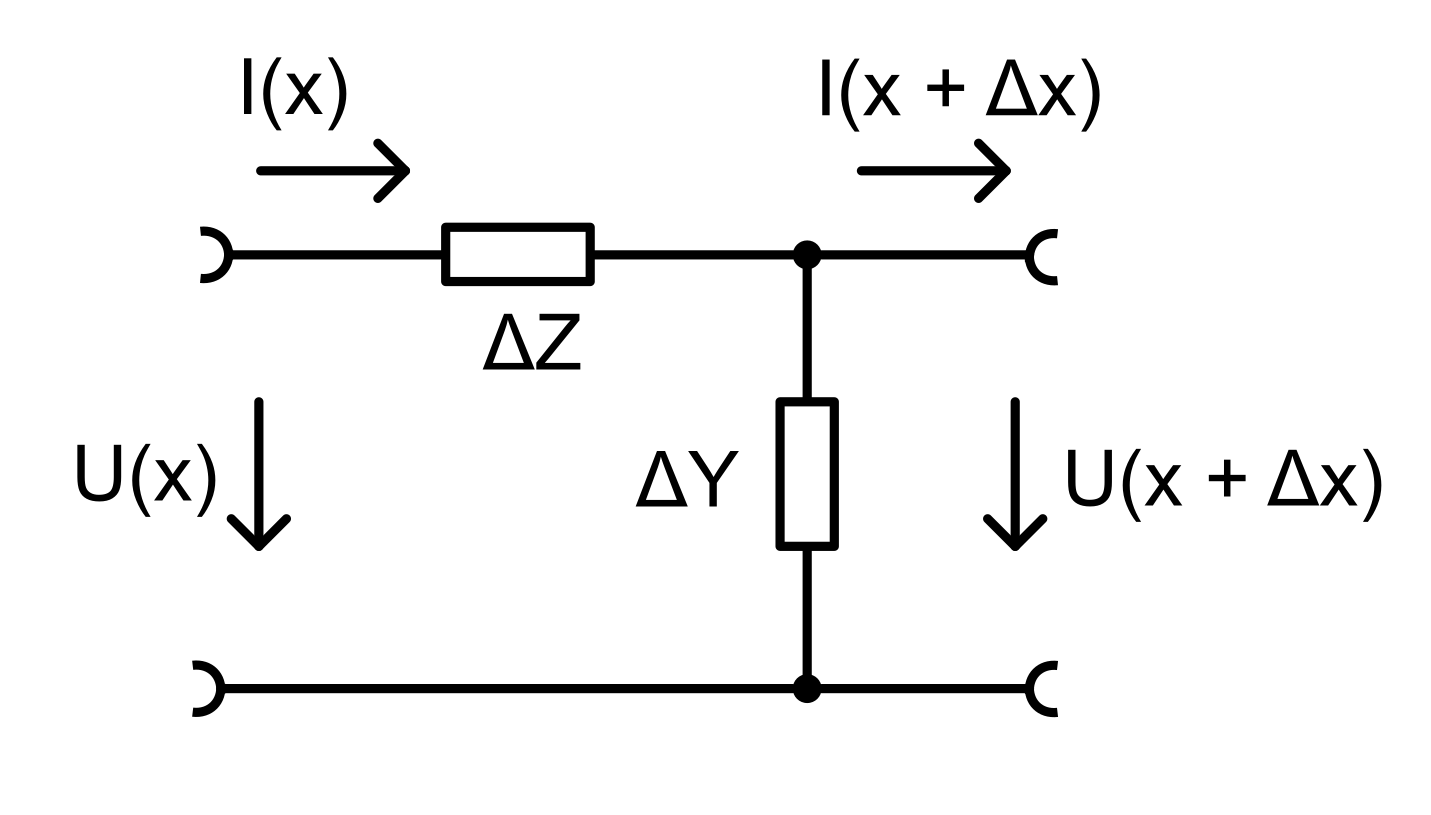
\includegraphics[width=0.8\textwidth]{ersatz_wellenausbreitung.png}
        \caption{Ersatzschaltbild zur Wellenausbreitung; Abbildung 1.3 \cite{Praktikumsanleitung}}
\end{figure}
Der Wellenwiderstand eines Kabels ist definiert als 
\begin{align} 
        Z=\dfrac{U_h\left(x\right)}{I_h\left(x\right)}=\dfrac{U_r\left(x\right)}{-I_r\left(x\right)}
,\end{align} 
mit $_h$ der Hinrichtung und $_r$ der Rückrichtung.
Im verlustfreien Fall ist $Z=\,\sqrt[]{\tfrac{L'}{C'}}$, also rein reell.
Für ein Koaxialkabel mit Innenradius $R_i$ und Außenradius $R_a$ gilt
\begin{align} 
        Z=Z_\text{frei}\cdot \dfrac{\ln\left(\tfrac{R_a}{R_i}\right)}{2\pi }
,\end{align} 
wobei $Z_\text{frei}=\,\sqrt[]{\tfrac{\mu _0}{\varepsilon _0}}=120\pi \,\SI{}{\ohm}$ der Wellenwiderstand des Vakuums ist.
\\\indent Es existieren drei verschiedene wichtige Möglichkeiten für den Abschlusswiderstand in einer Leitung.
\begin{enumerate}[label=--]
        \item Angepasster Abschluss: $R_A=Z,r=0,s=1,m=1$ 
        \item Offene Leitung: $R_A=\infty,r=+1,s=\infty,m=0$ 
        \item Kurzschluss: $R_A=0,r=-1,s=\infty,m=0$ 
\end{enumerate}
Hier beschreiben $R_A$ den Abschlusswiderstand, $r$ den Reflexionskoeffizienten, $s$ das Stehwellenverhältnis und $m$ den Anpassungsfaktor.

\newpage
\section{Voraufgaben}
\subsection{A}
Um große Verzögerungszeiten zu erreichen muss eine kleine Phasengeschwindigkeit sichergestellt werden, entsprechend große Permeabilität und Permitivität.

\subsection{B}
Wird die Verzögerungszeit über die Phasengeschwindigkeit geändert, so ändert sich auch der Wellenwiderstand, da diese Größen verschiedene Proportionalitäten besitzen
\begin{align} 
        v_{\text{ph}}\propto \dfrac{1}{\,\sqrt[]{L'C'}}\qquad Z\propto \,\sqrt[]{\dfrac{L'}{C'}}
.\end{align} 
Das Aufwickeln des Innenleiters um einen Ferritkern damit die Induktivität des Kabels gesteigert wird ändert den Wellenwiderstand nicht.

\subsection{C}
Sei ein Kabel abgeschlossen mit $R_A=Z$, findet keine Reflexion statt.
Alle Energie, die am Eingang des Kabels einläuft, wird am Kabelende vollständig an den Verbraucher $R_A$ abgegeben, da dieser wie eine Fortsetzung des Kabels aussieht.
Der Eingangswiderstand ist hier also unabhängig von der Länge des Kabels.

\subsection{D}
Sei ein verlustfreier idealer Leiter mit den Eigenschaften $\tfrac{R_A}{R_I}=2.3,\varepsilon _r=1.5$ und $\mu _r=1.5$.
Dann ist die Phasengeschwindigkeit
\begin{align} 
        v_{\text{ph}}&=\dfrac{c_0}{\,\sqrt[]{\varepsilon _r\mu _r}}=\dfrac{c_0}{1.5}\approx \SI{1.93e+8}{m.s ^{-1}}
,\end{align} 
der Wellenwiderstand
\begin{align} 
        Z=\,\sqrt[]{\dfrac{L'}{C'}}=\,\sqrt[]{\dfrac{\mu _r\mu _0}{\varepsilon _r\varepsilon _0}\dfrac{\ln^2\left(R_a/R_i\right)}{4\pi ^2}}\approx \SI{49.94}{\ohm}
\end{align} 
und die Verzögerung
\begin{align} 
        \Delta =\dfrac{1}{v_{\text{ph} }}=\dfrac{1.5}{c_0}\approx \SI{5.2e-9}{s.m ^{-1}}\approx \SI{5.2}{\nano s.m ^{-1}}
.\end{align} 


\newpage
\section{Auswertung}

\subsection{Versuchsaufgabe 1: Differenzierglied}
Wir erzeugen Impulse, indem wir ein Rechtecksignal mithilfe eines Differenzierglieds ableiten. Es sind 200 kHz bei 10 V eingestellt. Ein Ausschnitt ist in Abb. \ref{fig:1.1} gezeigt.
\begin{figure}[h]
        \centering
        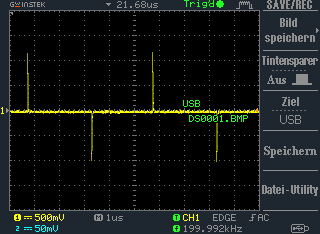
\includegraphics[width=0.8\textwidth]{data/DS0001.BMP.png}
        \caption{Impulse als Ableitung des Rechtecksignals}
		\label{fig:1.1}
\end{figure}
Wenn wir nun den eingebauten 2.2 k$\Omega$ Widerstand verwenden, sehen wir eine deutliche Verkleinerung des Rignals (betrachte die gelbe Skalar: 50 mV im Vergleich zu 500 mV von zuvor). Dieses ist wieder in Abb. \ref{fig:1.2} dargestellt. Zusätzlich können wir eine Abklinkzeit beobachten. Dies ist auch plausibel, da Widerstände Dämpfen, sowie die Konstruktion nicht mehr annähand Verlustfrei machen und so eine sichbare Verzögerung/Abklinkzeit hinzukommt.
\begin{figure}[h]
        \centering
        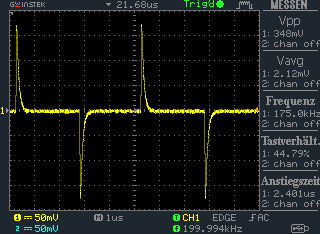
\includegraphics[width=0.8\textwidth]{data/DS0003.BMP.png}
        \caption{Impulse mit Widerstand}
		\label{fig:1.2}
\end{figure}
\subsection{Versuchsaufgabe 2: Impulse auf Kabeln}
Es wird eine Schaltung nach Abb. \ref{fig:2.1} aufgebaut, um Impulse an beiden Enden hin- und herlaufen zu lassen.
\begin{figure}[h]
        \centering
        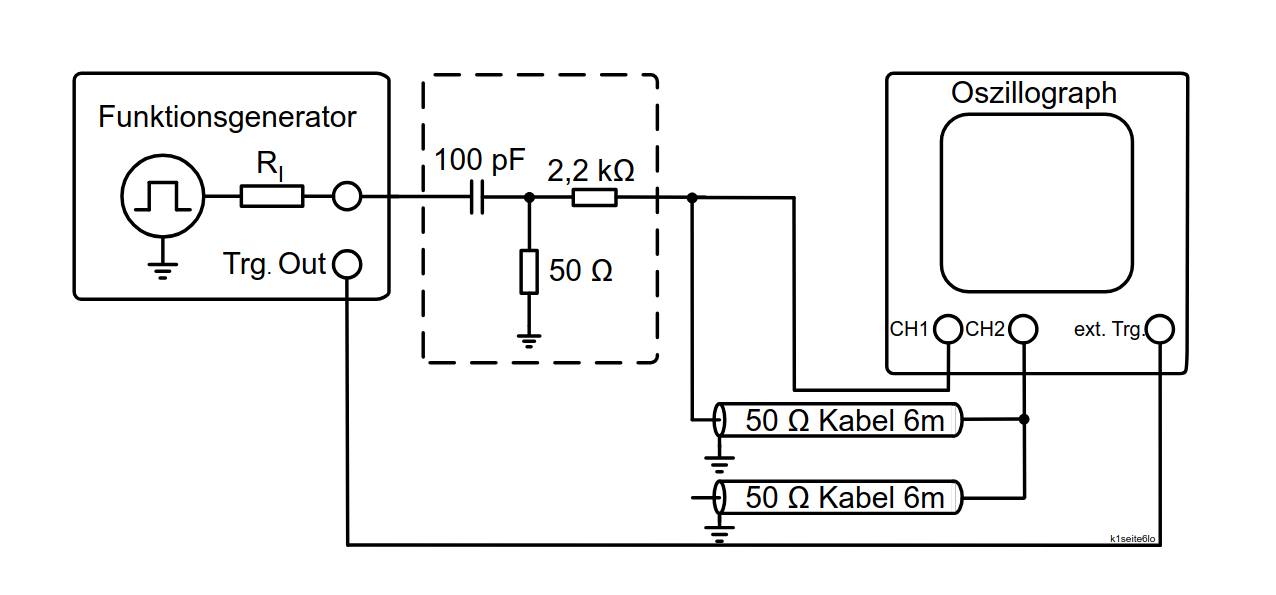
\includegraphics[width=0.8\textwidth]{Schaltung_offen.png}
        \caption{Schaltung mit offenen Enden}
		\label{fig:2.1}
\end{figure}
An dem Signalgenerator stellen wir 100 kHz und 20V ein.
\begin{figure}[h]
        \centering
        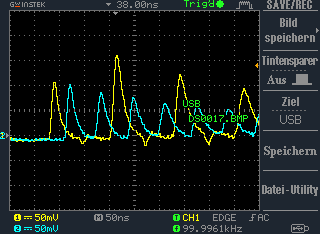
\includegraphics[width=0.8\textwidth]{data/DS0017.BMP.png}
        \caption{Schaltung mit offenen Enden}
		\label{fig:2.2}
\end{figure}
Bei dem Urspungssignal sehen wir, dass es mit einem größerem Peak und dann mit kleineren Peaks nachhallt. Das zweite Signal, welches durch die Kabel gedämpft wird, hier in blau in Abb. \ref{fig:2.2}, zieht um einen Versatz dem Ursprungssignal nach und beinhaltet zusätzlich die rückläufige Welle. So lassen sich pro Ursprungssignal, zwei weitere Peaks dem blauen Signal entnehmen. Die rückläufige Welle Entsteht aufgrund des offenen Leiter-Endes, welches als Glanzfläche, die einlaufende Welle phasengleich reflektiert. Einen Abstieg der Amplituden lässt sich aufgrund der Dämpfung - des Widerstands im Kabel - erklären.

\subsection{Versuchsaufabe 3: Leitungsabschluss, Verzögerungszeit}
Zur Untersuchng verschiedener Leitungsabschlüsse wird die Schaltung nach Abb. \ref{fig:3.1} konstruiert. 
\begin{figure}[h]
        \centering
        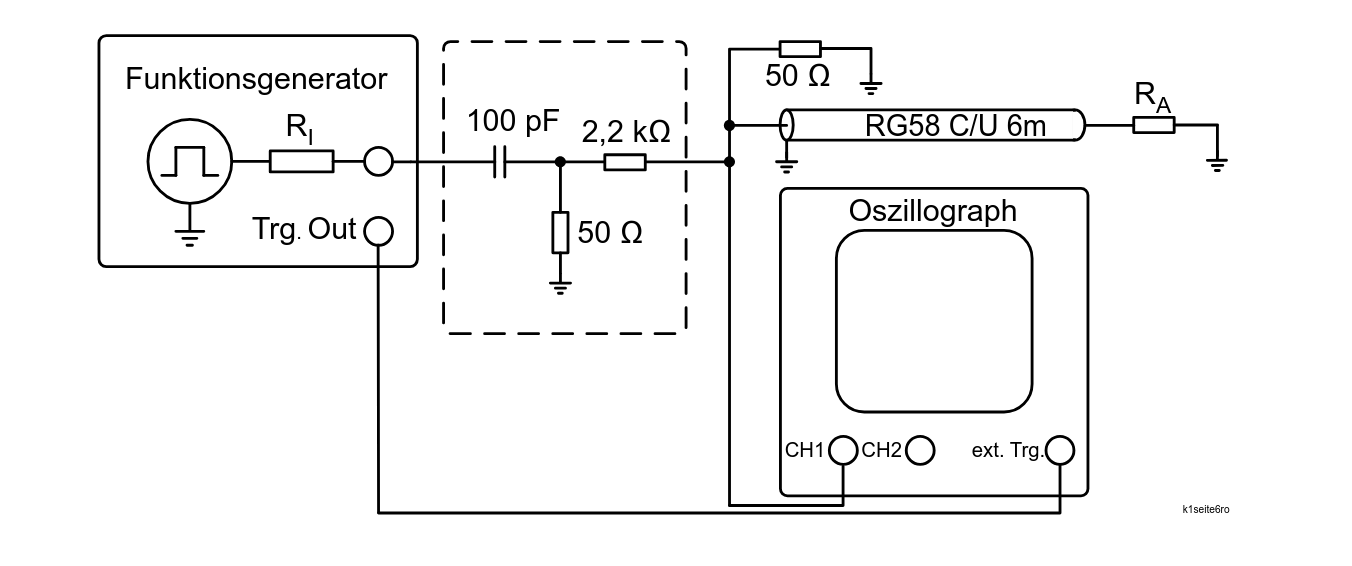
\includegraphics[width=0.8\textwidth]{Schaltung_Abschluss.png}
        \caption{Schaltung mit offenen Enden}
		\label{fig:3.1}
\end{figure}

Vorerst ist hierbei das Verzögerungskabel offen. Wir erhlaten die in Abb. \ref{fig:3.2} gezeigte Spannung.
\begin{figure}[h]
        \centering
        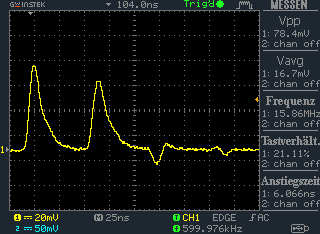
\includegraphics[width=0.8\textwidth]{data/DS0018.BMP.png}
        \caption{Einzelner Impuls mit Nachschwingung}
		\label{fig:3.2}
\end{figure}
\begin{figure}[h]
        \centering
        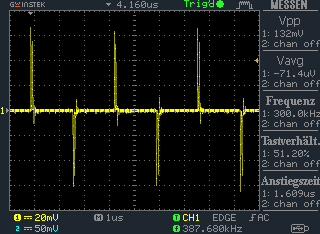
\includegraphics[width=0.8\textwidth]{data/DS0021.BMP.png}
        \caption{Mehrere Impulse mit Nachschwingung}
		\label{fig:3.3}
\end{figure}
Hierbei ist klar der eigentliche Impuls, sowie die Nachschwingung (zweiter Peak) zu erkennen.

Schließen wir nun das Kabel mit einem 50 $\Omega$ ab, so können wir in Abb. \ref{fig:3.4} erkennen, dass es keine Nachschwingung gibt und das Kabel aus der eigenen Sicht unendlich weitergeführt wird. 
\begin{figure}[h]
        \centering
        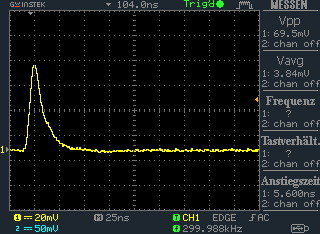
\includegraphics[width=0.8\textwidth]{data/DS0019.BMP.png}
        \caption{Einzelner Impuls ohne Nachschwingung}
		\label{fig:3.4}
\end{figure}
\begin{figure}[h]
        \centering
        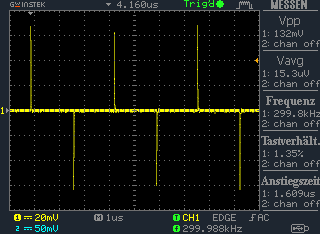
\includegraphics[width=0.8\textwidth]{data/DS0020.BMP.png}
        \caption{Mehrere Impulse ohne Nachschwingung}
		\label{fig:3.5}
\end{figure}

Lassen wir nun das Kabel in einem Kurzschluss enden, so kann man in Abb. \ref{fig:3.6} die rücklaufende gegenphasige Nachschwingung erkennen.
\begin{figure}[h]
        \centering
        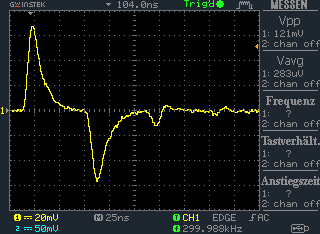
\includegraphics[width=0.8\textwidth]{data/DS0023.BMP.png}
        \caption{Einzelner Impuls mit gegenphasiger Nachschwingung}
		\label{fig:3.6}
\end{figure}
\begin{figure}[h]
        \centering
        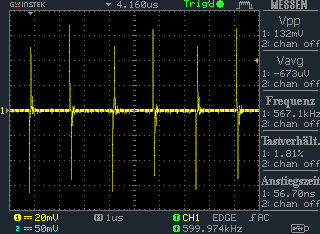
\includegraphics[width=0.8\textwidth]{data/DS0022.BMP.png}
        \caption{Mehrere Impulse mit gegenphasiger Nachschwingung}
		\label{fig:3.7}
\end{figure}
Diese gegenphasige Nachschiwngung ist aufgrund des kleineren Widerstandes zu erklären, da bei einem Kurzschluss der Widerstand praktisch Null und somit kleiner dem Wellenwiderstand ist. 




\clearpage
\listoffigures
\listoftables
\bibliographystyle{plain}
\bibliography{refs}

%}}}

\end{document}
